
\section{Session 4: Constrained optimization}
%------------------------------------------------%------------------------------------------------
In the previous section we have considered functions of several variables that are independent from each other. What happens if the variables are, however, not independent from each other? (see excellent material in \href{https://www.statslab.cam.ac.uk/~rrw1/}{Richard Weber's web site})

  \begin{center}
    
\includegraphics[width=0.7\textwidth]{../figures/mallorca.jpg}\newline
    What is the maximum height we can attain constrained to the trajectory of the road?
  \end{center}

%------------------------------------------------%------------------------------------------------
  Let us consider optimizing a function $f(x,y)$ (the height of the hill in the previous exemple) subject to the constrain $g(x,y)=c$ (the equation describing the path, the road).

  One can simply substitute $g(x,y)=c$ in $f(x,y)$, but this may not involve trivial algebra.

  Alternatively, let us consider the method of the Lagrange multipliers. To optimize $f(x,y)$ we require
  \[
    df=\frac{\partial f}{\partial x} dx +\frac{\partial f}{\partial y}dy=0
  \]
  we saw that if $dx$ and $dy$ were independent, $\frac{\partial f}{\partial x}=\frac{\partial f}{\partial y}=0$. But they are not here: they are constrained by $g(x,y)$, which is a constant:
  \[
    dg=\frac{\partial g}{\partial x} dx +\frac{\partial g}{\partial y}dy=0
  \]
  Let us consider a parameter $\lambda$ (the {\it Lagrange multiplier}) and obtain an expression for which $dx$ and $dy$ are independent:
  \[
    d(f+\lambda g)=(\frac{\partial f}{\partial x}+\lambda \frac{\partial g}{\partial x}) dx +(\frac{\partial f}{\partial y}+\lambda \frac{\partial g}{\partial y})dy=0
  \]
  Now:
  \begin{eqnarray*}
    \frac{\partial f}{\partial x}+\lambda \frac{\partial g}{\partial x} &=&0\\
    \frac{\partial f}{\partial y}+\lambda \frac{\partial g}{\partial y} &=&0\\
    g(x,y)&=&c
  \end{eqnarray*}
  are sufficient to find $\lambda$, $x^*$ and $y^*$.

%------------------------------------------------%------------------------------------------------
  \begin{center}
  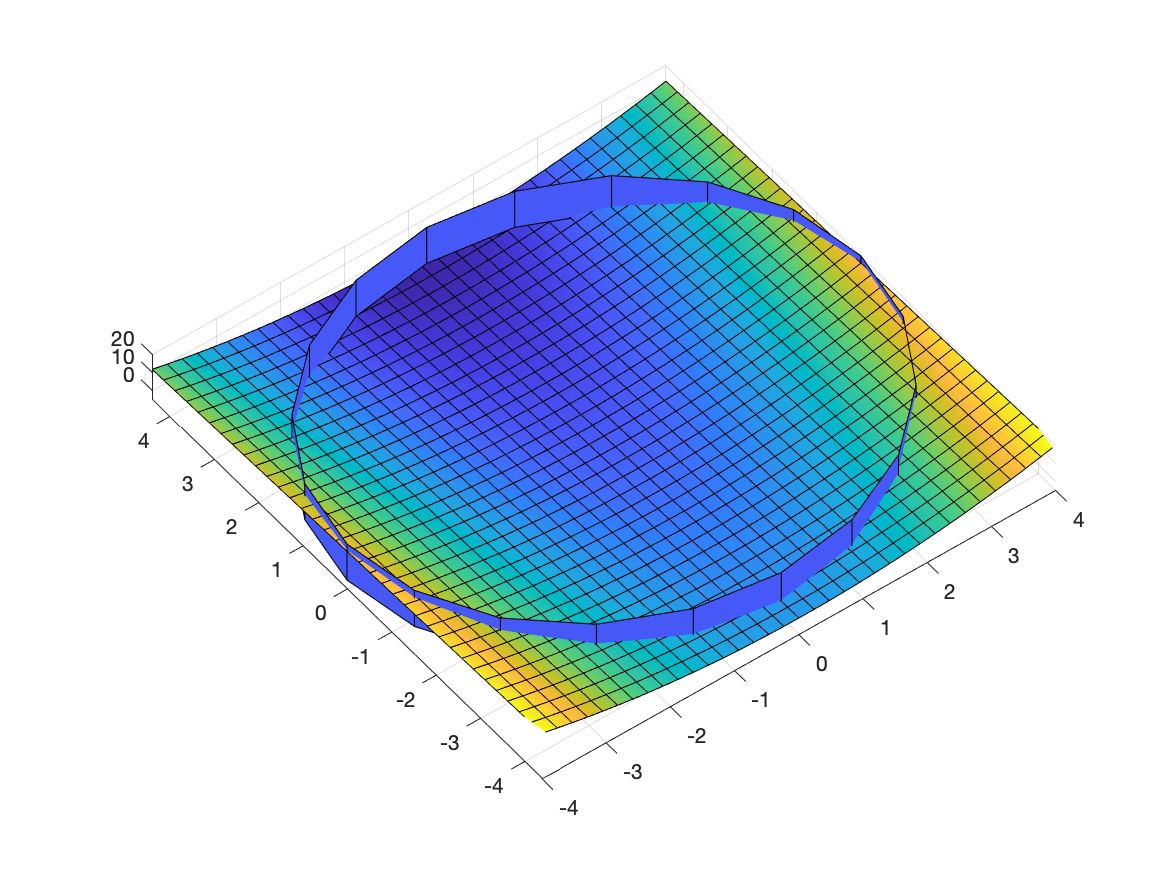
\includegraphics[width=0.4\textwidth]{../figures/Lagrangex2minusy.png}
  \end{center}
  \begin{Exercise}
  Find the optimal values of the function $f(x,y)=x^2-y$ constrained within the circumference $x^2+y^2=4$. (note that, interestingly, in the optimal value $x^*$ we will get a gradient for the constraint that is parallel to the gradient of the function: $\grad f(x^*)=\lambda^* \grad g(x^*)$).
\end{Exercise}
%------------------------------------------------%------------------------------------------------
  The general problem we study takes the form
  \begin{center}
  \begin{tabular}{cc}
    maximize & $f(x)$ \\
    subject to & $\begin{cases}x\in X\\g(x)=b\end{cases}$
  \end{tabular}
\end{center}
where
  \begin{center}
  \begin{tabular}{rl}
    $x \in \mathbf{R}^n$ & ($n$ decision variables)\\
    $f: \mathbf{R}^n \rightarrow \mathbf{R}$ & (objective function)\\
    $X \subseteq  \mathbf{R}^n$ & (regional constraints) \\
    $\begin{rcases}
      g: \mathbf{R}^n \rightarrow \mathbf{R}^m\\
      b \subseteq \mathbf{R}^m
    \end{rcases}$ & ($m$ functional constraints)\\
  \end{tabular}
\end{center}
If the constraint is $g(x)\leq b$ we introduce a {\bf slack variable} $z$ and write:
\[g(x)+z=b, \, z\geq0\]
Regional and functional constraints define the {\bf feasible set} for $x$

%------------------------------------------------%------------------------------------------------

  In the Lagrange approach, the constrained maximization (minimization) problem is rewritten as a Lagrange function 
  
  \[L(x,\lambda)=f(x)-\lambda g(x)\]
  
  whose optimal point is a saddle point, i.e. a global maximum (minimum) over the domain of the choice variables and a global minimum (maximum) over the multipliers.

  Let us take this example:
  \begin{center}
  \begin{tabular}{cc}
    maximize & $f(x)=x_1-x_2-2x_3$ \\
    subject to & $\begin{cases}x_1+x_2+x_3=5\\x_1^2+x_2^2=4\\x=(x_1,x_2,x_3)\in \mathbf{R}^3\end{cases}$
  \end{tabular}
\end{center}
\begin{enumerate}
  \item We write the Lagrangian as (note we have two constraints):
  \begin{eqnarray*}
    L(x,\lambda)&=&x_1-x_2-2x_3-\lambda_1 (x_1+x_2+x_3-5)-\lambda_2(x_1^2+x_2^2-4)\\
    &=& [x_1(1-\lambda_1)-\lambda_2x_1^2]+[x_2(-1-\lambda_1)-\lambda_2x_2^2]+[x_3(-2-\lambda_1)]\\
    &&+5\lambda_1+4\lambda_2
  \end{eqnarray*}
  \item We want to minimize the Lagrangian subject to the regional constraints $x=(x_1,x_2,x_3)\in \mathbf{R}^3$.
  \item We find the values $\lambda$ such that will define a feasible set
  \[
  Y=\left\{\lambda: \underbrace{\mathrm{min}}_{x\in  \mathbf{R}^3} L(x,\lambda) >-\infty \right\}
  \]
  So, we only consider the values of $\lambda$ for which we obtain a finite minimum. In the example
  \[
  Y=\left\{\lambda: \lambda_1=-2, \lambda_2<0 \right\}
  \]
  \item For $\lambda \in Y$, the minimum will be obtained at some $x(\lambda)$ (that depends on $\lambda$ in general). Here, $x(\lambda)=(3/2\lambda_2,1/2\lambda_2,x_3)^T$.
  \item Finally, we find a $\lambda$ value that provides a feasible value $x(\lambda)$. Here
  \[
    x_1^2+x_2^2=4 \Rightarrow \lambda_2 = -\sqrt{5/8}
  \]
  So, $x^*$ is optimal:
  \[
    x^* =(-3\sqrt{2/5},-\sqrt{2/5},5+4\sqrt{2/5})^T; \, \lambda^*=(-2,-\sqrt{5/8})^T
  \]
\end{enumerate}


\begin{Exercise}
  Use the Lagrange multipliers to solve this problem:
  \begin{center}
    \begin{tabular}{cc}
      minimize & $f(x,y)=x^2y$ \\
      subject to & $x^2+y^2=1$
    \end{tabular}
  \end{center}
\end{Exercise}
%------------------------------------------------%------------------------------------------------
% https://en.wikipedia.org/wiki/Karush%E2%80%93Kuhn%E2%80%93Tucker_conditions
  \footnote{\url{https://people.maths.bris.ac.uk/~maxmr/opt/kt1.pdf}}
  \footnote{\url{https://www.cmi.ac.in/~madhavan/courses/dmml2018/literature/Lagrangian_Methods_for_Constrained_Optimization.pdf}}

  Let us consider a general optimization problem with constraints: let $f:\mathbf{R}^n \rightarrow \mathbf{R}$ be the objective function and $\uvec{g}:\mathbf{R}^n \rightarrow \mathbf{R}^m$ a set of constraint functions ($\uvec{g}(\uvec{x})=(g_1(\uvec{x}),\ldots,g_m(\uvec{x}))$ with $\uvec{x}=(x_1,\ldots,x_n)$. We want to obtain
  \begin{center}
  Min $f(\uvec{x})$ such that $\uvec{g}(\uvec{x})\geq 0$
\end{center}
  \begin{theorem}
    If $\uvec{x}^*$ is a local minimum for the optimisation problem and the constraints $\uvec{g}(\uvec{x})\geq 0$ are satisfied at $\uvec{x}^*$, then $\uvec{x}^*$ must satisfy:
    \begin{eqnarray*}
      \grad f({\uvec{x}})&=&\lambda_1 \grad g_1(\uvec{x})+\cdots+\lambda_m \grad g_m(\uvec{x})\\
      0&=&\lambda_1  g_1(\uvec{x})=\cdots=\lambda_m  g_m(\uvec{x})\\
      0&\leq&\uvec{g}(\uvec{x})
    \end{eqnarray*}
  \end{theorem}

%------------------------------------------------%------------------------------------------------


  \begin{Exercise}
     Consider this NLO problem\cite{carter_operations_2019}:
    \begin{center}
     \begin{tabular}{cc}
      maximize & $f(x,y)=x^2y+2y^2$ \\
      subject to & $\begin{cases}x+3y\leq 9\\x+2y\leq 8\\3x+2y\leq 18\\0\leq x \leq 5\\0\leq y \leq 2\end{cases}$
    \end{tabular}
  \end{center}
    Solve the program graphically- Begin at point $(0,0)$ and check the gradient. Check the KKT conditions. If they are not satisfied, find an improving direction in the feasible region.
  \end{Exercise}


%------------------------------------------------%------------------------------------------------
  To better understand these exercises, you can make use of \href{https://www.geogebra.org/3d?lang=en}{geogebra}.
\begin{Exercise}
  Is it possible to maximize $f(x,y)=xy$ subject to $100 \geq x+y$ and $x\leq 40$?
  % solution: not necessarily, feasible region is not bound. In fact it is not possible
\end{Exercise}
\begin{Exercise}
  %https://personal.math.ubc.ca/~israel/m340/kkt2.pdf
  What about maximizing $f(x,y)=xy$ subject to $x+y^2\leq 2$ and $x,y \geq 0$?
\end{Exercise}
%https://www.sfu.ca/~wainwrig/Econ400/lecture-notes-Kuhntucker.pdf

%-----